\documentclass{article}

\usepackage[english]{babel}
\usepackage[a4paper,top=2cm,bottom=2cm,left=3cm,right=3cm,marginparwidth=1.75cm]{geometry}

% Useful packages
\usepackage[backend=biber, sorting=nyt, style=authoryear-ibid]{biblatex}
\usepackage[inkscapeformat=png]{svg}
\usepackage[outputdir=pdf]{minted}
\usepackage{graphicx}
\graphicspath{ {figures/} }
\usepackage[colorlinks=true, allcolors=blue]{hyperref}
\usepackage{parskip}
%\usepackage{lipsum}
\usepackage{setspace}
\doublespacing
\usepackage{multicol}
\usepackage{multirow}
\usepackage{fontspec}
\usepackage{fontawesome5}
\usepackage{amsmath}
\usepackage{csquotes}

% Document style
%\usepackage[utf8]{inputenc} % Required for inputting international characters
%\usepackage[T1]{fontenc} % Output font encoding for international characters
%\usepackage{palatino} % Use the Palatino font
%\usepackage{microtype} % Improves spacing
%\usepackage[bf,sf,center]{titlesec} % Required for modifying section titles - bold, sans-serif, centered
%\usepackage{fancyhdr} % Required for modifying headers and footers
%\fancyhead[L]{\textsf{\rightmark}} % Top left header
%\fancyhead[R]{\textsf{\leftmark}} % Top right header
%\renewcommand{\headrulewidth}{1.4pt} % Rule under the header
%\fancyfoot[C]{\textbf{\textsf{\thepage}}} % Bottom center footer
%\renewcommand{\footrulewidth}{1.4pt} % Rule under the footer
%\pagestyle{fancy} % Use the custom headers and footers throughout the document

% Appendix dictionary template: print each word on the page
% \markboth{}{} prints the first word on the page in the top left header and the last word in the top right
%\newcommand{\entry}[4]{\markboth{#1}{#1}\textbf{#1}\ {(#2)}\ \textit{#3}\ $\bullet$\ {#4}}
\newcommand{\entry}[2]{\markboth{#1}{#1}\textbf{#1}\ $\bullet$\ {#2}}


%----------------------------------------------------------------------------------------
%  The completed Case Study Report (no more than 5000 words) 
%    must be submitted on Weblearn by Friday 10th of May 2024 at 15:00.
%
%  A single pdf of your report saved with the appropriate filename (see below). The filenames should be of the form: A B C.pdf
%
%  A = Your ID, B = Case Study Report , C = YY (last 2 digits of the year) For example : 12345678 Case Study Report 24.pdf
%
%  DONOTPUTDATAinthereport(onlythefirst20casesintheAppendix).
%
%  Anyfigureyouuseshouldhaveacaptionbelowlike:
%     Figure 1: Showing the linear regression of y against time. (You should refer to Figure 1 in the text).
%
%  Youshouldonlyputtheimportantresultsorfiguresinthereportandcommentonthem.
%
%  PutPAGENumbersintoyourreport.
%
%  The report does not have to be long. Extensive output without comments will get little credit. Your comments and explanation are most important.
%  
%----------------------------------------------------------------------------------------

%\bibliography{references}
\addbibresource{references.bib}

\title{MA7007 - Statistical Modelling and Forecasting Case Study Report 2023-2024}
\author{Stuart Kingham: ID 21014912}

\begin{document}
\doublespacing

%\begin{center}
%{\LARGE Case Study Report 2023-2024}
%\end{center} 
%\vspace*{\fill}


%\maketitle
\begin{titlepage}
  \topskip0pt
  \vspace*{\fill}
  \begin{center}
       \vspace*{1cm}

       {\LARGE Case Study Report 2023-2024}

       \vspace*{1cm}
       {\large \textbf{Statistical Analysis of Data Sets}}
       
       %\vspace{1.5cm}

       \vfill

       \textbf{Stuart Kingham: ID 2101491}

       \vfill
                        
       \vspace{0.8cm}
     
       %\includegraphics[width=0.4\textwidth]{university}

       MM7007: Statistical Modelling and Forecasting\\
       School of Computing and Digital Media\\
       London Metropolitan University\\
       May 10, 2024
            
  \end{center}
  \vspace*{\fill}
\end{titlepage}

\pagebreak

\begin{abstract}
  Abstract
\end{abstract}

\newpage

\singlespacing 
\tableofcontents
\listoffigures
\listoftables
\doublespacing

\pagenumbering{roman}
\pagenumbering{arabic}
\newpage

\section{Introduction}

Recently in the Harvard Business Review (HBR), \textcite{Coppersmith1997} identified the challenges regarding cyber-security oversight by company
boards.   In the HBR report survey, boards are saying that they are not seeing eye-to-eye with their CISOs, with one example being that while
\enquote{65\% of board members think their organization is at risk of a material cyber-attack, only 48\% of CISOs share that view.}

\begin{figure}[!ht] % Single column figure
  %\includegraphics[width=0.95\textwidth]{statistic_id267132_annual-amount-of-financial-damage-caused-by-reported-cybercrime-in-us-2001-2022.png}\hfill
  \includesvg[width=0.95\textwidth]{Lattice-reduction}\hfill
  \caption{Latice Reduction \autocite{Wikipedia:2021}  Source: Wikipedia.}
  \label{fig:lattice-reduction}
\end{figure}



\section{First data set}

Fitting distributions to the data.

(a) Comment on the different distributions you are using.
(b) Which distribution did you choose?
(c) Give reasons why you chose the distribution in part (b).
(d) Plot the fitted distribution and comment.
(e) State the fitted parameter values of the final chosen model



\section{Second data set}

Centile estimation \ldots

\subsection{Distribution Overview}

where the smoothing for age uses the P-splines function pb(), i.e. pb(age), for the predictors for parameter $\mu$, $\sigma$ and $\nu$.

How many degrees of freedom were used for smoothing in the model? Use the function edf()or edfAll().

When selecting the final model, especially after using smoothing techniques like P-splines (pb()), it's crucial to balance fit and complexity. Here are factors to consider in justifying your model choice:

*    Goodness of Fit: Use diagnostic plots and goodness-of-fit statistics to ensure the model adequately captures the relationship between grip strength and age.

*    Complexity vs. Simplicity: A model with more degrees of freedom can capture more complex relationships but risks overfitting. Ensure the EDF values suggest a model complex enough to capture essential patterns without overfitting.

*    Comparison with Alternative Models: If applicable, compare your chosen model with alternatives using information criteria like AIC or BIC, which penalize model complexity.

*    Interpretability: Ensure the model remains interpretable. While more complex models might provide a marginally better fit, they should not do so at the expense of being understandable.

The BCCG distribution is chosen for its flexibility in modeling skewed data, which is often encountered in physical measurements like grip strength. By adjusting for age with P-splines, the model can flexibly accommodate nonlinear age effects on the distribution parameters of grip strength, making it a powerful approach for analyzing such data.

4.5 Choosing an appropriate distribution
The choice of an appropriate response distribution is based on how well the distribution
fits the data as judged by (i) the generalized Akaike information criterion GAIC, (ii)
the prediction global deviance VDEV, (iii) the residuals, or (iv) other criteria.

4.5.1 Generalized Akaike information criterion (GAIC)
The fitted global deviance is defined as minus twice the fitted log likelihood (defined in Section 10.2):
$GDEV = -2 \sum^{n}_{i=1} log f(yi | j\Theta)$ (4.2)

where $\Theta = (\mu; \sigma; \nu; \tau )$ are the fitted parameters, which for regression models depend
on the explanatory variables. The generalized Akaike information criterion, GAIC, is
defined as $GAIC(\kappa) = GDEV + \kappa . df$ (4.3)

where $df$ is the effective degrees of fr
eedom used for the fitted model and $\kappa$ is a penalty
for each degree of freedom used. The AIC and BIC/SBC are special cases of the GAIC
when $\kappa = 2$ and $\kappa = log n$, respectively, i.e.

$AIC = GDEV + 2 df$

$SBC = GDEV + log n . df$

These measures are discussed in Chapter 3 of Stasinopoulos et al. [2017] and in Section 11.5.5.

\subsection{Fitting the Distributions}

\subsubsection{grip against age. Note that there is no need to power transform the agein this data set. Explain why.}

Why No Power Transformation is Necessary:
*    Linearity: If the relationship between age and grip strength is linear or close to linear, applying a transformation to age would not yield any significant benefits in terms of linear regression modeling or interpretation.
    
*    Variability: Power transformations are also used to stabilize variance across the range of predictor variables. If the variance of grip strength is relatively constant across ages, then transforming age wouldn't help in stabilizing variance.
    
*    Normality of Residuals: Another reason for transformations could be to achieve normality of residuals in regression modeling. If the residuals from a model with age predicting grip strength are already approximately normally distributed, a transformation is unnecessary.
    
*    Simplicity: Avoiding unnecessary transformations keeps the model simpler and makes interpretation more straightforward. If a simple model without transformation provides satisfactory results, it's often preferred for ease of explanation and understanding.

\subsubsection{How many degrees of freedom were used for smoothing in the model? }

Interpreting the Effective Degrees of Freedom:

*    EDF Near 1: If the effective degrees of freedom for a parameter is close to 1, it suggests that the model is applying very little smoothing to that parameter. This can imply a linear relationship between the parameter and the predictors.

*    EDF Greater Than 1: An EDF significantly greater than 1 indicates more complex relationships are being modeled, with the splines applying more smoothing. This is often necessary when the relationship between the response and predictors is nonlinear or when there's a varying effect of predictors across the range of the data.

*    High EDF: Very high EDF values may signal overfitting, where the model is too closely fitting the idiosyncrasies of the sample data rather than capturing the underlying population trends.

The mu, sigma, nu, and tau parameters represent different aspects of the distribution being modeled:

*   mu ($\mu$): The location parameter (central tendency).
*   sigma ($\sigma$): The scale parameter (dispersion or variability).
*   nu ($\nu$) and 
*   tau ($\tau$): Parameters that control the shape of the distribution, including skewness and kurtosis.

Choosing between the BCT and BCPE models, and interpreting their parameters' EDFs, depends on the fit quality, predictive performance, and the complexity trade-off. This process is crucial for understanding how age influences grip strength across its distribution and ensuring the model's generalizability.

\subsubsection{What are the effective degrees of freedom fitted for the parameters? Try to interpret the effective degrees of freedom.}


\subsubsection{Investigate the residuals from the fitted models}

(c) Use residual diagnostics for checking the model

\subsubsection{Investigate the residuals from the fitted models}

*    Residual Plots: You're looking for patterns or systematic deviations from zero. Ideally, residuals should be randomly distributed around zero without clear patterns.

*    Worm Plots (WP): These plots should ideally resemble a straight line. Curvature or deviations from the line indicate potential issues with the model's fit to the data, such as non-normality or heteroscedasticity.

*    Q-Statistics (Q.stats()): This provides a summary of the quantiles of the residuals compared to the expected distribution. Significant deviations can indicate that the model's assumptions about the distribution of residuals may not hold.

When using these diagnostic tools, it's important to consider them collectively rather than relying on a single method. Each tool can highlight different aspects of the model fit and potential areas for improvement.

\subsubsection{Selection of Distribution}
(d) Comment on how you selected your final model.


The GAIC is a variant of the Akaike Information Criterion (AIC) that allows for a more flexible penalization of model complexity and is particularly useful in comparing models fitted with the same dataset but different distributions or complexities.

Interpreting GAIC

When comparing models with GAIC, the model with the lowest GAIC value is generally considered the best among the set, as it strikes the most favorable balance between model fit and complexity. The GAIC penalizes models more heavily for additional parameters than the traditional AIC does, making it particularly useful for models that might overfit the data with too many parameters or excessive flexibility.

*    Lower GAIC: Indicates a model that has a better trade-off between goodness-of-fit and complexity, suggesting it might generalize better to new data.

*    Comparing Values: The absolute value of the GAIC is not interpretable on its own; it's the relative differences between the GAIC scores of the models that inform model selection. A difference of more than a few points is generally considered meaningful.

By evaluating the GAIC values for your three models, you can make an informed decision about which model provides the best fit to your data without unnecessarily increasing model complexity. This is particularly useful in your case, where you're fitting different distributions and considering different forms of the response variable's relationship with predictors.




\subsubsection{centile plot for the fitted models: compare them.}

(e) Comment on the final centile plots.


Interpreting the Comparison:

*    Overlap and Divergence: Overlapping lines suggest agreement between models in estimating grip strength across age centiles. Divergence indicates differences in how models estimate grip strength at various ages, potentially due to differences in distributional assumptions or how well each model captures the variability in the data.

*    Model Fit and Data Representation: This visual comparison can help assess which model might provide a better fit or more accurately represent the underlying trends and variations in your data. For example, if one model's centiles follow the data more closely or seem to capture the trend without overfitting, it might be preferable.

By comparing these centile plots, you get a visual representation of how each model performs across the range of ages, which can inform your decision on the best model for your analysis based on how well they fit the centiles to the observed data.


\section{Third data set}

This section of the report is an analysis of real credit card default data, \citetitle{Cheng:2026} \cite{Cheng:2026},
from a Taiwan bank in 2005.

The data contains a snapshot of client information showing those who have defaulted on their repayments, along with their
credit limit and history of their bill amounts, re-payment amounts and outstanding payments, along with certain client demographics, such
as age, marriage status, education level and gender.

The aim for the analysis here was to develop a robust predictive model using \texttt{GAMLSS} that captures the complex dynamics in the
probability of default among credit card holders.  This question seeks to explore the efficacy of GAMLSS, which allows for the
flexible modeling of distributions and can accommodate the skewness and kurtosis inherent in financial datasets. 

This data set had been investigated by other researchers \cite{Yeh:2009} so we have a baseline for comparing our results against other
methodologies.

A note in here; the size and poor correlations of the explanatory variables with the response meant that the analysis and
fitting stages were very time consuming and error prone.  

\subsection{Data Schema}

\begin{verbatim}
# Variable Name Role	Type	  Demographic	      Description	Units	Missing Values
# ID           ID	  Integer				                              no
# X1	       Feature	  Integer		                LIMIT_BAL		      no
# X2	       Feature	  Factor	  Sex	            SEX		              no
# X3	       Feature	  Factor	  Education Level	EDUCATION		      no
# X4	       Feature	  Factor	  Marital Status	MARRIAGE		      no
# X5	       Feature	  Integer	  Age	            AGE		              no
# X6	       Feature	  Double		                PAY_0		          no
# X7	       Feature	  Double		                PAY_2		          no
# X8	       Feature	  Double		                PAY_3		          no
# X9	       Feature	  Double		                PAY_4		          no
# X10	      Feature	  Double		                PAY_5		          no
# X11	      Feature	  Double		                PAY_6		          no
# X12	      Feature	  Double		                BILL_AMT1		      no
# X13	      Feature	  Double		                BILL_AMT2		      no
# X14	      Feature	  Double		                BILL_AMT3		      no
# X15	      Feature	  Double		                BILL_AMT4		      no
# X16	      Feature	  Double		                BILL_AMT5		      no
# X17	      Feature	  Double		                BILL_AMT6		      no
# X18	      Feature	  Double		                PAY_AMT1		      no
# X19	      Feature	  Double		                PAY_AMT2		      no
# X20	      Feature	  Double		                PAY_AMT3		      no
# X21	      Feature	  Double		                PAY_AMT4		      no
# X22	      Feature	  Double		                PAY_AMT5		      no
# X23	      Feature	  Double		                PAY_AMT6		      no
# Y	          Target	  Binary		                default.payment.next.month		no
\end{verbatim}

\subsubsection{Preliminary Analysis}

The data are clean and reliable with no missing values.  The csv file contains 30000 rows of data with:
one identity column; 23 explanatory variables and; the response
variable \texttt{default.payment.next.month}.


\begin{figure}[H]
  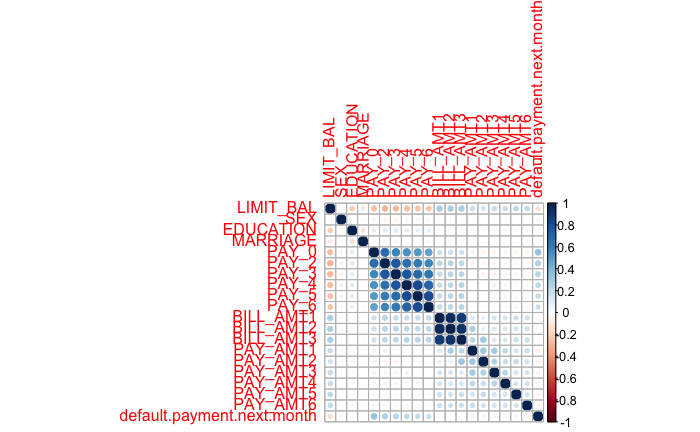
\includegraphics{q3_data_corr.png}
  \caption{Correlation analysis of the credit card default variables}
\end{figure}

The correlation between any of the variables is quite low, making the building of a robust model difficult.

\subsection{Statistical Model}

Our baseline BI model is build with all explanatory variable:
\begin{verbatim}
mbi <- gamlss(default.payment.next.month~LIMIT\_BAL+PAY\_0+PAY\_2+PAY\_3+PAY\_4+PAY\_5+PAY\_6+AGE+
                factor(EDUCATION)+factor(SEX)+factor(MARRIAGE)+BILL\_AMT1+PAY\_AMT1+BILL\_AMT2+PAY\_AMT2+
                BILL\_AMT3+PAY\_AMT3+BILL\_AMT4+PAY\_AMT4+BILL\_AMT5+PAY\_AMT5+BILL\_AMT6+PAY\_AMT6, 
              family=BI, # BI is for Binomial distribution
              data=cc\_train)
\end{verbatim}


\subsubsection{Selecting a Distribution}

The response variable \textbf{\texttt{default.payment.next.month}} is a binary value on the default event: one as 'Yes', zero as 'No'.
Binomial models are our only alternatives here. Manually fitting the different families show that the standard \textbf{Binomial Model}
\verb|BI| gives the best AIC scoring.  This is fortunate as with testing a large number of explanatory variable using stepwise
algorithms is already computationally expensive.


\subsection{Model Diagnostics}

\begin{figure}[H]
  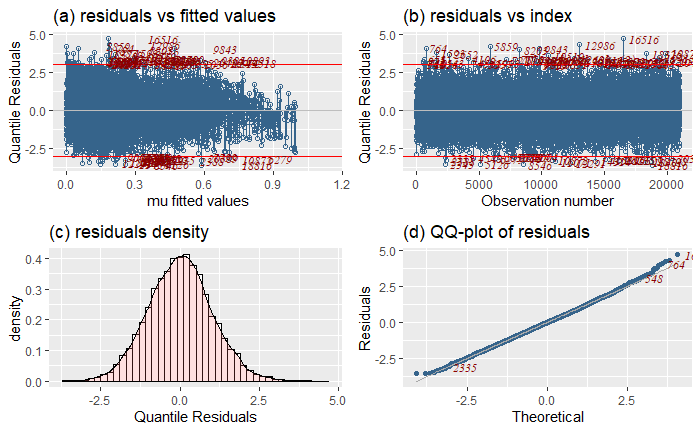
\includegraphics{q3_mbi_plot.png}
  \caption{BI residuals worm plot for credit card defaults}
\end{figure}

In this residuals analysis we start to see the problems before us.  The residuals worm plot has a high curvature and large extreme
values.

\begin{figure}[H]
  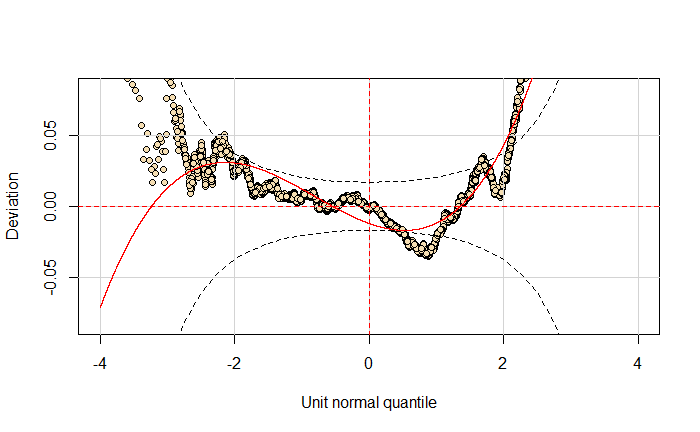
\includegraphics{q3_mbi_wp.png}
  \caption{BI residuals worm plot for credit card defaults}
\end{figure}

Using the \verb|stepGAICAll.B| function we find an improved AIC, but the worm plot is not much improved.

Using spline smoothing improves the situation markedly.

\begin{figure}[H]
  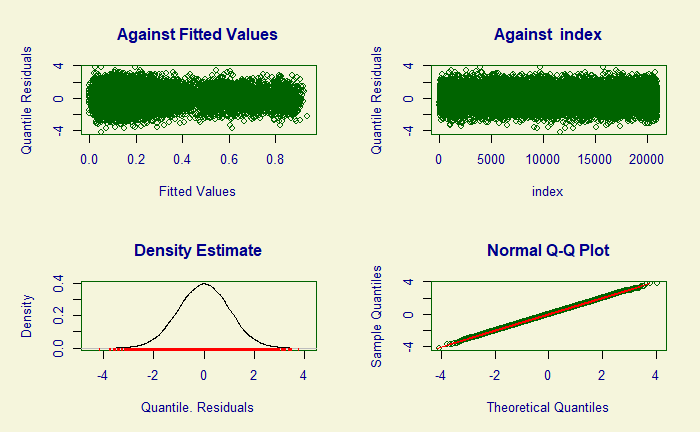
\includegraphics{q3_mbi4_plot.png}
  \caption{BI with smoothing and stepwise residuals plot}
\end{figure}

\begin{figure}[H]
  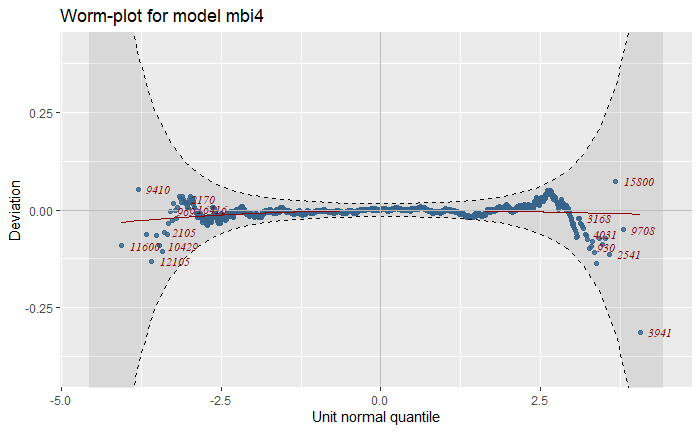
\includegraphics{q3_mbi4_wp.png}
  \caption{BI with smoothing and stepwise residuals worm plot}
\end{figure}



\subsection{Model Prediction}


\begin{verbatim}
library(pROC)
predicted_probabilities <- predict(mbi4, newdata = cc_validation, type = "response")
actual_values <- cc_validation$default.payment.next.month
roc_curve <- roc(cc_validation$default.payment.next.month, predicted_probabilities)
plot(roc_curve, main = "ROC Curve")


cor(predicted_probabilities, actual_values)
[1] 0.4489414
\end{verbatim}

\begin{figure}[H]
  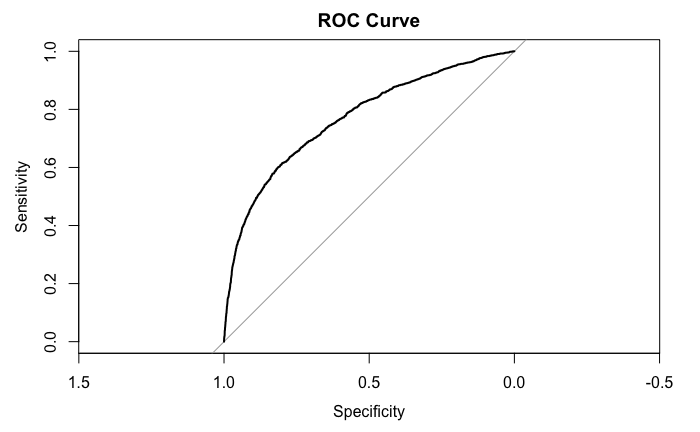
\includegraphics{q3_predict_roc.png}
  \caption{BI with smoothing and stepwise residuals worm plot}
\end{figure}

The correlation value is low.  This needs more work.


\section{PeerReview}

(a) Choose one from a selection of student work on the third data set.

(b) Write a short critique on the adequacy of the work. You should look at:

\begin{itemize}
\item thequalityoftheexplorativeanalysisofthedataset
\item thechoiceofthedistributionfortheresponse(target)variable 
\item  themethodforselectingandcheckingthemodel
\item  theinterpretationoftheresults
\end{itemize}

(c) Give a grade [A, B, C, D, E, F] representing your estimation of the value of the work.



\pagebreak

\section{Conclusion}

\subsection{Summary of Findings}

Recap the key points discussed in the paper.

\subsection{Personal Insight}

Present your personal viewpoint developed through the research and implementation.


\subsection{Future Work}

Suggest areas for further research or potential improvements in the method.

\subsection{Final Thoughts}

Conclude with the significance of your findings for the field of cryptography.


\pagebreak

\printbibliography

\pagebreak

\appendix

\section{Appendix: Full Maple Code}

Description of implementation, etc
 
\subsection{RSA Implementation}

\begin{listing}[!ht]
\inputminted{python}{tex/code/coppersmith_rsa.mw}
\caption{Maple RSA Implementation code}
\label{listing:1}
\end{listing}

\subsection{Stereotyped Message Attack}


                   

\end{document}

%%% Local Variables:
%%% mode: latex
%%% TeX-master: t
%%% End:
